\documentclass[12pt,a4paper]{article}
\usepackage{charter}
%\usepackage[latin1]{inputenc}
\usepackage[left=1.50cm, right=1.50cm, top=1.20cm]{geometry}
\usepackage{amsmath}
\usepackage{amsfonts}
\usepackage{amssymb}
\usepackage{graphicx}
\usepackage{textcomp}
\renewcommand{\baselinestretch}{1.5}
\usepackage{listings}
\usepackage{xcolor}
\definecolor{listinggray}{gray}{0.9}
\definecolor{lbcolor}{rgb}{0.9,0.9,0.9}
\usepackage{float}
\usepackage{CJKutf8}
\usepackage{textcomp}
%\lstset{
%	backgroundcolor=\color{lbcolor},
%	tabsize=4,    
%	%   rulecolor=,
%	language=[GNU]C++,
%	basicstyle=\scriptsize,
%	upquote=true,
%	aboveskip={1.5\baselineskip},
%	columns=fixed,
%	showstringspaces=false,
%	extendedchars=false,
%	breaklines=true,
%	prebreak = \raisebox{0ex}[0ex][0ex]{\ensuremath{\hookleftarrow}},
%	frame=single,
%	numbers=left,
%	showtabs=false,
%	showspaces=false,
%	showstringspaces=false,
%	identifierstyle=\ttfamily,
%	keywordstyle=\color[rgb]{0,0,1},
%	commentstyle=\color[rgb]{0.026,0.112,0.095},
%	stringstyle=\color[rgb]{0.627,0.126,0.941},
%	numberstyle=\color[rgb]{0.205, 0.142, 0.73},
%	%        \lstdefinestyle{C++}{language=C++,style=numbers}?.
%}
%\lstset{
%	backgroundcolor=\color{lbcolor},
%	tabsize=4,
%	language=C++,
%	captionpos=b,
%	tabsize=3,
%	frame=lines,
%	numbers=left,
%	numberstyle=\tiny,
%	numbersep=5pt,
%	breaklines=true,
%	showstringspaces=false,
%	basicstyle=\footnotesize,
%	%  identifierstyle=\color{magenta},
%	keywordstyle=\color[rgb]{0,0,1},
%	commentstyle=\color{Darkgreen},
%	stringstyle=\color{red}
%}

\lstdefinestyle{customc}{
	belowcaptionskip=1\baselineskip,
	aboveskip={1.2\baselineskip},
	breaklines=true,
	frame=lines,
	numbers=left,
	xleftmargin=\parindent,
	language=C++,
	showstringspaces=false,
	basicstyle=\sffamily,%,\ttfamily,
	keywordstyle=\bfseries\color{green!40!black},
	commentstyle=\itshape\color{purple!40!black},
	identifierstyle=\color{blue},
	stringstyle=\color{orange},
	breaklines=true,
	postbreak=\raisebox{0ex}[0ex][0ex]{\ensuremath{\color{red}\hookrightarrow\space}}
}

\lstdefinestyle{customasm}{
	belowcaptionskip=1\baselineskip,
	frame=L,
	xleftmargin=\parindent,
	language=[x86masm]Assembler,
	basicstyle=\footnotesize\ttfamily,
	commentstyle=\itshape\color{purple!40!black},
}

\lstset{escapechar=@,style=customc}

\begin{document}
\section{Solution}
\subsection{60}
\begin{CJK}{UTF8}{gbsn}
这道题是让求出n个数字的第k个排列组合,由于其特殊性,我们不用将所有的排列组合的情况都求出来,然后返回其第k个,
我们可以只求出第k个排列组合即可,那么难点就在于如何知道数字的排列顺序,
首先我们要知道当n = 3时,其排列组合共有$3! = 6$种,当n = 4时,其排列组合共有$4! = 24$种,
我们就以n = 4, k = 17的情况来分析,所有排列组合情况如下:
\end{CJK}
\begin{center}
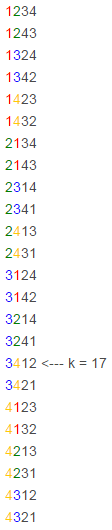
\includegraphics{0060.png}
\end{center}
\begin{CJK}{UTF8}{gbsn}
我们可以发现,每一位上1,2,3,4分别都出现了6次,当第一位上的数字确定了,后面三位上每个数字都出现了2次,当第二位也确定了,后面的数字都只出现了1次,当第三位确定了,那么第四位上的数字也只能出现一次,那么下面我们来看k = 17这种情况的每位数字如何确定,由于k = 17是转化为数组下标为16:
\par
最高位可取1,2,3,4中的一个,每个数字出现$3!= 6$次,所以k = 16的第一位数字的下标为$16 / 6 = 2$,即3被取出
\par
第二位此时从1,2,4中取一个,$k = 16$是此时的$k_1 = 16 \% (3!)$ = 4,而剩下的每个数字出现$2!= 2$次,所以第二数字的下标为$4 / 2 = 2$,即4被取出
\par
第三位此时从1,2中去一个,$k_1 = 4$是此时的$k_2 = 4 \% (2!) = 0$,而剩下的每个数字出现$1!= 1$次,所以第三个数字的下标为 $0 / 1 = 0$,即1被取出
\par
第四位是从2中取一个,$k_2 = 0$是此时的$k_3 = 0 \% (1!) = 0$,而剩下的每个数字出现$0!= 1$次,所以第四个数字的下标为$0 / 1= 0$,即2被取出
\par
那么我们就可以找出规律了
\end{CJK}
\par
$a_1 = k / (n - 1)!$
\par
$k_1 = k$
\par
$a_2 = k_1 / (n - 2)!$
\par
$k_2 = k_1 \% (n - 2)!$
\par
\dots
\par
$a_{n-1} = k_{n-2} / 1!$
\par
$k_{n-1} = k_{n-2} / 1!$
\par
$a_n = k_{n-1} / 0!$
\par
$k_n = k_{n-1} \% 0!$
\begin{lstlisting}
string getPermutation( int n, int k ) {
	string res;
	string num = "123456789";
	vector<int> f( n, 1 );
	for ( int i = 1; i < n; ++i ) f[i] = f[i - 1] * i;
	--k;
	for ( int i = n; i >= 1; --i ) {
		int j = k / f[i - 1];
		k %= f[i - 1];
		res.push_back( num[j] );
		num.erase( j, 1 );
	}
	return res;
}
\end{lstlisting}


\subsection{61}
\begin{enumerate}
\item
\begin{CJK}{UTF8}{gbsn}
这道旋转链表的题和之前那道 Rotate Array 旋转数组 很类似,但是比那道要难一些,因为链表的值不能通过下表来访问,只能一个一个的走,我刚开始拿到这题首先想到的就是用快慢指针来解,快指针先走k步,然后两个指针一起走,当快指针走到末尾时,慢指针的下一个位置是新的顺序的头结点,这样就可以旋转链表了,自信满满的写完程序,放到OJ上跑,以为能一次通过,结果跪在了各种特殊情况,首先一个就是当原链表为空时,直接返回NULL,还有就是当k大于链表长度和k远远大于链表长度时该如何处理,我们需要首先遍历一遍原链表得到链表长度n,然后k对n取余,这样k肯定小于n,就可以用上面的算法了
\end{CJK}
\begin{lstlisting}
ListNode *rotateRight( ListNode *head, int k ) {
	if ( !head ) return NULL;
	int n = 0;
	ListNode *cur = head;
	while ( cur ) {
		++n;
		cur = cur->next;
	}
	k %= n;
	ListNode *fast = head, *slow = head;
	for ( int i = 0; i < k; ++i ) {
		if ( fast ) fast = fast->next;
	}
	if ( !fast ) return head;
	while ( fast->next ) {
		fast = fast->next;
		slow = slow->next;
	}
	fast->next = head;
	fast = slow->next;
	slow->next = NULL;
	return fast;
}
\end{lstlisting}
\item
\begin{CJK}{UTF8}{gbsn}
这道题还有一种解法,跟上面的方法类似,但是不用快慢指针,一个指针就够了,
原理是先遍历整个链表获得链表长度n,然后此时把链表头和尾链接起来,
在往后走$n - k \% n$个节点就到达新链表的头结点前一个点,这时断开链表即可
\end{CJK}
\begin{lstlisting}
ListNode *rotateRight( ListNode *head, int k ) {
	if ( !head ) return NULL;
	int n = 1;
	ListNode *cur = head;
	while ( cur->next ) {
		++n;
		cur = cur->next;
	}
	cur->next = head;
	int m = n - k % n;
	for ( int i = 0; i < m; ++i ) {
		cur = cur->next;
	}
	ListNode *newhead = cur->next;
	cur->next = NULL;
	return newhead;
}
\end{lstlisting}
\end{enumerate}


\subsection{62}
\begin{CJK}{UTF8}{gbsn}
这道题让求所有不同的路径的个数,一开始还真把我难住了,因为之前好像没有遇到过这类的问题,所以感觉好像有种无从下手的感觉。
在网上找攻略之后才恍然大悟,原来这跟之前那道 Climbing Stairs 爬梯子问题 很类似,那道题是说可以每次能爬一格或两格,问到达顶部的所有不同爬法的个数。而这道题是每次可以向下走或者向右走,
求到达最右下角的所有不同走法的个数。那么跟爬梯子问题一样,我们需要用动态规划Dynamic Programming来解,
我们可以维护一个二维数组dp,其中dp[i][j]表示到当前位置不同的走法的个数,
然后可以得到递推式为: dp[i][j] = dp[i - 1][j] + dp[i][j - 1],
这里为了节省空间,我们使用一维数组dp,一行一行的刷新也可以,代码如下
\end{CJK}
\begin{lstlisting}
int uniquePaths( int m, int n ) {
	vector<int> dp( n, 1 );
	for ( int i = 1; i < m; ++i ) {
		for ( int j = 1; j < n; ++j ) {
			dp[j] += dp[j - 1];
		}
	}
	return dp[n - 1];
}
\end{lstlisting}

\subsection{63}
\begin{enumerate}
\item
\begin{CJK}{UTF8}{gbsn}
这道题是之前那道 Unique Paths 不同的路径 的延伸,在路径中加了一些障碍物,
还是用动态规划Dynamic Programming来解,不同的是当遇到为1的点,
将该位置的dp数组中的值清零,其余和之前那道题并没有什么区别
\end{CJK}
\begin{lstlisting}
int uniquePathsWithObstacles( vector<vector<int>>& obstacleGrid ) {
	if ( obstacleGrid.empty() || obstacleGrid[0].empty() || obstacleGrid[0][0] == 1 ) return 0;
	vector<vector<int> > dp( obstacleGrid.size(), vector<int>( obstacleGrid[0].size(), 0 ) );
	for ( int i = 0; i < obstacleGrid.size(); ++i ) {
		for ( int j = 0; j < obstacleGrid[i].size(); ++j ) {
			if ( obstacleGrid[i][j] == 1 ) dp[i][j] = 0;
			else if ( i == 0 && j == 0 ) dp[i][j] = 1;
			else if ( i == 0 && j > 0 ) dp[i][j] = dp[i][j - 1];
			else if ( i > 0 && j == 0 ) dp[i][j] = dp[i - 1][j];
			else dp[i][j] = dp[i - 1][j] + dp[i][j - 1];
		}
	}
	return dp.back().back();
}
\end{lstlisting}
\item
\begin{CJK}{UTF8}{gbsn}
或者我们也可以使用一维dp数组来解,省一些空间
\end{CJK}
\begin{lstlisting}
int uniquePathsWithObstacles( vector<vector<int> > &obstacleGrid ) {
	if ( obstacleGrid.empty() || obstacleGrid[0].empty() ) return 0;
	int m = obstacleGrid.size(), n = obstacleGrid[0].size();
	if ( obstacleGrid[0][0] == 1 ) return 0;
	vector<int> dp( n, 0 );
	dp[0] = 1;
	for ( int i = 0; i < m; ++i ) {
		for ( int j = 0; j < n; ++j ) {
			if ( obstacleGrid[i][j] == 1 ) dp[j] = 0;
			else if ( j > 0 ) dp[j] += dp[j - 1];
		}
	}
	return dp[n - 1];
}
\end{lstlisting}
\end{enumerate}

\subsection{64}
\begin{CJK}{UTF8}{gbsn}
这道题跟之前那道 Dungeon Game 地牢游戏 没有什么太大的区别,
都需要用动态规划Dynamic Programming来做,这应该算是DP问题中比较简单的一类,
我们维护一个二维的dp数组,其中dp[i][j]表示当前位置的最小路径和,
递推式也容易写出来 dp[i][j] = grid[i][j] + min(dp[i - 1][j],dp[i][j-1]), 反正难度不算大
\end{CJK}
\begin{lstlisting}
int minPathSum( vector<vector<int> > &grid ) {
	int m = grid.size(), n = grid[0].size();
	int dp[m][n];
	dp[0][0] = grid[0][0];
	for ( int i = 1; i < m; ++i ) dp[i][0] = grid[i][0] + dp[i - 1][0];
	for ( int i = 1; i < n; ++i ) dp[0][i] = grid[0][i] + dp[0][i - 1];
	for ( int i = 1; i < m; ++i ) {
		for ( int j = 1; j < n; ++j ) {
			dp[i][j] = grid[i][j] + min( dp[i - 1][j], dp[i][j - 1] );
		}
	}
	return dp[m - 1][n - 1];
}
\end{lstlisting}

\subsection{65}
\begin{enumerate}
\item
\begin{CJK}{UTF8}{gbsn}
首先,从题目中给的一些例子可以分析出来,我们所需要关注的除了数字以外的特殊字符有空格, 小数点, 自然数 ``e/E'', 还要加上正负号 ``+/-'',
除了这些字符需要考虑意外,出现了任何其他的字符,可以马上判定不是数字。下面我们来一一分析这些出现了也可能是数字的特殊字符:
\begin{enumerate}
\item 空格: 空格分为两种情况需要考虑,一种是出现在开头和末尾的空格,一种是出现在中间的字符。出现在开头和末尾的空格不影响数字,而一旦中间出现了空格,则立马不是数字。解决方法:预处理时去掉字符的首位空格,中间再检测到空格,则判定不是数字。
\item 小数点: 小数点需要分的情况较多,首先的是小数点只能出现一次,但是小数点可以出现在任何位置,开头(".3"), 中间("1.e2"), 以及结尾("1." ), 而且需要注意的是,小数点不能出现在自然数 ``e/E'' 之后,如 "1e.1" false, "1e1.1" false。还有,当小数点位于末尾时,前面必须是数字,如 "1."  true," -." false。解决方法:开头中间结尾三个位置分开讨论情况。

3. 自然数 'e/E':自然数的前后必须有数字,即自然数不能出现在开头和结尾,如 "e" false,  ".e1" false, "3.e" false, "3.e1" true。而且小数点只能出现在自然数之前,还有就是自然数前面不能是符号,如 "+e1" false, "1+e" false. 解决方法:开头中间结尾三个位置分开讨论情况。

4. 正负号 '+/-",正负号可以再开头出现,可以再自然数e之后出现,但不能是最后一个字符,后面得有数字,如  "+1.e+5" true。解决方法:开头中间结尾三个位置分开讨论情况。

 

下面我们开始正式分开头中间结尾三个位置来讨论情况:

1. 在讨论三个位置之前做预处理,去掉字符串首尾的空格,可以采用两个指针分别指向开头和结尾,遇到空格则跳过,分别指向开头结尾非空格的字符。

2. 对首字符处理,首字符只能为数字或者正负号 '+/-",我们需要定义三个flag在标示我们是否之前检测到过小数点,自然数和正负号。首字符如为数字或正负号,则标记对应的flag,若不是,直接返回false。

3. 对中间字符的处理,中间字符会出现五种情况,数字,小数点,自然数,正负号和其他字符。

若是数字,标记flag并通过。

若是自然数,则必须是第一次出现自然数,并且前一个字符不能是正负号,而且之前一定要出现过数字,才能标记flag通过。

若是正负号,则之前的字符必须是自然数e,才能标记flag通过。

若是小数点,则必须是第一次出现小数点并且自然数没有出现过,才能标记flag通过。

若是其他,返回false。

4. 对尾字符处理,最后一个字符只能是数字或小数点,其他字符都返回false。

若是数字,返回true。

若是小数点,则必须是第一次出现小数点并且自然数没有出现过,还有前面必须是数字,才能返回true。
\end{CJK}
\begin{lstlisting}
bool canJump( int A[], int n ) {
	vector<int> dp( n, 0 );
	for ( int i = 1; i < n; ++i ) {
		dp[i] = max( dp[i - 1], A[i - 1] ) - 1;
		if ( dp[i] < 0 ) return false;
	}
	return dp[n - 1] >= 0;
}
\end{lstlisting}
\item
\begin{CJK}{UTF8}{gbsn}
还有一种省空间的DP方法,维护一个常量maxIdx,表示最远能到达的位置,
遍历数组中每一个数字,如果当前坐标大于maxIdx或者maxIdx已经抵达最后一个位置则跳出循环,
否则就更新maxIdx的值为其和i + A[i]中的较大值,其中i + A[i]表示当前位置能到达的最大位置
\end{CJK}
\begin{lstlisting}
bool canJump( int A[], int n ) {
	int maxIdx = 0;
	for ( int i = 0; i < n; ++i ) {
		if ( i > maxIdx || maxIdx >= n - 1 ) break;
		maxIdx = max( maxIdx, i + A[i] );
	}
	return maxIdx >= n - 1;
}
\end{lstlisting}
\end{enumerate}

\subsection{56}
\begin{enumerate}
\item
\begin{CJK}{UTF8}{gbsn}
这道和之前那道 Insert Interval 插入区间 很类似,这次题目要求我们合并区间,
之前那题明确了输入区间集是有序的,而这题没有,
所有我们首先要做的就是给区间集排序,由于我们要排序的是个结构体,
所以我们要定义自己的comparator,才能用sort来排序,
我们以start的值从小到大来排序,排完序我们就可以开始合并了,
首先把第一个区间存入结果中,然后从第二个开始遍历区间集,
如果结果中最后一个区间和遍历的当前区间无重叠,直接将当前区间存入结果中,
如果有重叠,将结果中最后一个区间的end值更新为结果中最后一个区间的end和当前end值之中的较大值,
然后继续遍历区间集,以此类推可以得到最终结果
\end{CJK}
\begin{lstlisting}
class Solution {
public:
	static bool comp( const Interval &a, const Interval &b ) {
		return (a.start < b.start);
	}
	vector<Interval> merge( vector<Interval> &intervals ) {
		vector<Interval> res;
		if ( intervals.empty() ) return res;
		sort( intervals.begin(), intervals.end(), comp );
		res.push_back( intervals[0] );
		for ( int i = 1; i < intervals.size(); ++i ) {
			if ( res.back().end >= intervals[i].start ) {
				res.back().end = max( res.back().end, intervals[i].end );
			}
			else {
				res.push_back( intervals[i] );
			}
		}
		return res;
	}
};
\end{lstlisting}
\item
\begin{CJK}{UTF8}{gbsn}
这道题还有另一种解法,这个解法直接调用了之前那道题 Insert Interval 插入区间 的函数,
由于插入的过程中也有合并的操作,所以我们可以建立一个空的集合,
然后把区间集的每一个区间当做一个新的区间插入结果中,也可以得到合并后的结果
\end{CJK}
\begin{lstlisting}
// Using insert method
class Solution {
public:
	vector<Interval> merge( vector<Interval> &intervals ) {
		vector<Interval> res;
		for ( int i = 0; i < intervals.size(); ++i ) {
			res = insert( res, intervals[i] );
		}
		return res;
	}
	vector<Interval> insert( vector<Interval> &intervals, Interval newInterval ) {
		vector<Interval> res = intervals;
		vector<Interval>::iterator it = res.begin();
		int overlap = 0;
		while ( it != res.end() ) {
			if ( newInterval.end < it->start ) break;
			else if ( newInterval.start > it->end ) {}
			else {
				newInterval.start = min( newInterval.start, it->start );
				newInterval.end = max( newInterval.end, it->end );
				++overlap;
			}
			++it;
		}
		if ( overlap != 0 ) it = res.erase( it - overlap, it );
		res.insert( it, newInterval );
		return res;
	}
};
\end{lstlisting}
\end{enumerate}

\subsection{57}
\begin{enumerate}
\item
\begin{CJK}{UTF8}{gbsn}
这道题让我们在一系列非重叠的区间中插入一个新的区间,可能还需要和原有的区间合并,
那么我们需要对给区间集一个一个的遍历比较,那么会有两种情况,重叠或是不重叠,
不重叠的情况最好,直接将新区间插入到对应的位置即可,重叠的情况比较复杂,
有时候会有多个重叠,我们需要更新新区间的范围以便包含所有重叠,
而且最后处理的时候还需要删除原区间集中所有和新区间重叠的区间,然后插入新区间即可。具体思路如下:
\begin{itemize}
\item 对区间集中每个区间进行遍历
\begin{itemize}
\item 如果新区间的末尾小于当前区间的开头,则跳出循环
\item 如果新区间的开头大于当前区间的末尾,不作处理
\item 如果新区间和当前区间有重叠,则更新新区间的开头为两者最小值,新区间的末尾为两者最大值,重叠数加一
\item 指针移向下一个区间
\end{itemize}
\item 如果重叠数大于0,则删除掉所有的重叠区间
\item 插入新区间到对应的位置
\end{itemize}
\end{CJK}
\begin{lstlisting}
vector<Interval> insert( vector<Interval> &intervals, Interval newInterval ) {
	vector<Interval> res = intervals;
	int i = 0, overlap = 0, n = res.size();
	while ( i < n ) {
		if ( newInterval.end < res[i].start ) break;
		else if ( newInterval.start > res[i].end ) {}
		else {
			newInterval.start = min( newInterval.start, res[i].start );
			newInterval.end = max( newInterval.end, res[i].end );
			++overlap;
		}
		++i;
	}
	if ( overlap > 0 ) res.erase( res.begin() + i - overlap, res.begin() + i );
	res.insert( res.begin() + i - overlap, newInterval );
	return res;
}
\end{lstlisting}
\item
\begin{CJK}{UTF8}{gbsn}
对Iterator Pattern比较熟悉的也可应用Iterator来求解,本质还是一样的,只是写法略有不同
\end{CJK}
\begin{lstlisting}
vector<Interval> insert( vector<Interval> &intervals, Interval newInterval ) {
	vector<Interval> res = intervals;
	vector<Interval>::iterator it = res.begin();
	int overlap = 0;
	while ( it != res.end() ) {
		if ( newInterval.end < it->start ) break;
		else if ( newInterval.start > it->end ) {}
		else {
			newInterval.start = min( newInterval.start, it->start );
			newInterval.end = max( newInterval.end, it->end );
			++overlap;
		}
		++it;
	}

	if ( overlap != 0 ) it = res.erase( it - overlap, it );
	res.insert( it, newInterval );
	return res;
}
\end{lstlisting}
\end{enumerate}

\subsection{58}
\begin{CJK}{UTF8}{gbsn}
这道题难度不是很大。先对输入字符串做预处理,
去掉开头和结尾的空格,然后用一个计数器来累计非空格的字符串的长度,遇到空格则将计数器清零
\end{CJK}
\begin{lstlisting}
int lengthOfLastWord( const char *s ) {
	int len = strlen( s );
	int left = 0;
	int right = len - 1;
	int count = 0;
	while ( s[left] == ' ' ) ++left;
	while ( s[right] == ' ' ) --right;
	for ( int i = left; i <= right; ++i ) {
		if ( s[i] == ' ' ) count = 0;
		else ++count;
	}
	return count;
}
\end{lstlisting}

\subsection{59}
\begin{CJK}{UTF8}{gbsn}
此题跟之前那道 Spiral Matrix 螺旋矩阵 本质上没什么区别,
就相当于个类似逆运算的过程,这道题是要按螺旋的顺序来填数,
由于给定矩形是个正方形,我们计算环数时用n / 2来计算,
若n为奇数时,此时最中间的那个点没有被算在环数里,所以最后需要单独赋值,
还是下标转换问题是难点,参考之前 Spiral Matrix 螺旋矩阵 的讲解来转换下标吧,
\end{CJK}
\begin{lstlisting}
vector<vector<int> > generateMatrix( int n ) {
	vector<vector<int> > res( n, vector<int>( n, 1 ) );
	int val = 1, p = n;
	for ( int i = 0; i < n / 2; ++i, p -= 2 ) {
		for ( int col = i; col < i + p; ++col )
			res[i][col] = val++;
		for ( int row = i + 1; row < i + p; ++row )
			res[row][i + p - 1] = val++;
		for ( int col = i + p - 2; col >= i; --col )
			res[i + p - 1][col] = val++;
		for ( int row = i + p - 2; row > i; --row )
			res[row][i] = val++;
	}
	if ( n % 2 != 0 ) res[n / 2][n / 2] = val;
	return res;
}
\end{lstlisting}
\end{document}